\newpage
\section{Design patterns}

\subsection{Strutturali}
\subsubsection{Facade}
\textbf{Scopo}	Permette, attraverso un'interfaccia più semplice, l'accesso a sottosistemi che espongono interfacce complesse e molto diverse tra loro, nonché a blocchi di codice complessi. Questo rende una libreria più facile da capire, usare e testare, inoltre permette di diminuire le dipendenze tra sottosistemi senza nascondere le funzionalità di basso livello.
\\
\textbf{Motivazione}	L'utilizzo del pattern \textit{Facade\ped{G}} permette di nascondere la complessità del'operazione. Quando un sistema complesso viene strutturato in sottosistemi, le dipendenze rischiano di aumentare in modo consistente. Applicare il pattern \textit{Facede\ped{G}} aiuta a diminuire queste dipendenze. Il sottosistema possederà un'interfaccia semplificata che il \textit{client\ped{G}} utilizza anziché dover gestire numerosi oggetti. Utilizzare il pattern \textit{Facade\ped{G}} promuove un accoppiamento debole tra sottosistema ed i \textit{client\ped{G}}, che comporta una maggiore flessibilità nello sviluppo: è possibile modificare il sottosistema senza che i \textit{client\ped{G}} debbano adeguarsi a loro volta. \\
Ciononostante i \textit{client\ped{G}} possono comunque accedere alle funzionalità di basso livello ed utilizzare le classi del sottosistema.
\\
\textbf{Applicabilità}	Il pattern \textit{Facade\ped{G}} si usa nei seguenti casi:
	\begin{itemize}
		\item Si vuole fornire una singola interfaccia semplice per un sottosistema complesso;
		\item Si vuole promuovere il disaccoppiamento tra sottosistemi e \textit{client\ped{G}}, semplificando le dipendenze;
		\item Si vuole stratificare un sistema: è possibile definire una classe \textit{Facade\ped{G}} come punto d'ingresso per ogni livello di sottosistema. In questo modo, se vi sono dipendenze fra sottosistemi, essi possono comunicare fra loro attraverso la propria \textit{Facade\ped{G}}.
	\end{itemize}
\textbf{Utilizzo}

\subsection{Creazionali}
\subsubsection{Dependecy Injection}
\textbf{Scopo}	Semplificare lo sviluppo e rendere più testabile un software di grandi dimensioni. Il pattern \textit{Dependency Injection\ped{G}} separa il codice della componente dal codice che si occupa di risolvere le dipendenze con altre componenti.
\\ 
\textbf{Motivazione}	Lasciare al componente il compito di risolvere le proprie dipendenze, creando gli oggetti necessari al suo funzionamento, aumenta l'accoppiamento tra le componenti e rende più difficoltoso progettare i test di unità.
\\ Con questo pattern invece è possibile esprimere le dipendenze in modo dichiarativo e utilizzare un oggetto \textit{contenitore} per risolverle dinamicamente a \textit{runtime\ped{G}}. In questo modo è possibile scegliere anche quale componente iniettare in base allo stato del programma.
\\
\textbf{Applicabilità}	Questo pattern viene utilizzato dalla maggior parte dei \textit{framework\ped{G}} moderni. In particolare, \textit{AngularJS\ped{G}} offre il servizio \texttt{injector} che permette di invocare delle funzioni iniettando al loro interno degli oggetti.
\\
\textbf{Utilizzo}
\\
\textbf{Struttura}	I componenti coinvolti nel \textit{Dependency Injection} sono:
	\begin{itemize}
		\item Un \textit{client\ped{G}} che viene creato e riceve le dipendenze;
		\item Un \textit{contenitore} che si occupa di creare il \textit{client\ped{G}} e di iniettarvi le dipendenze;
		\item Un \textit{servizio} che deve essere iniettato al \textit{client\ped{G}}.
	\end{itemize}
Nello specifico di \textit{AngularJS\ped{G}} \texttt{Injector} funziona da \textit{contenitore} che si occupa di risolvere le dipendenze. I \textit{client\ped{G}} sono rappresentati dalle funzioni che costruiscono i componenti dell'applicazione, tipicamente \textit{controller\ped{G}} o \textit{service\ped{G}}. Il \textit{servizio} è un oggetto \textit{service} che può essere definito dall'utente oppure uno di quelli resi disponibili da \textit{AngularJS\ped{G}}.
\label{Struttura logica del pattern Dependency Injection}
\begin{figure}
	\centering
	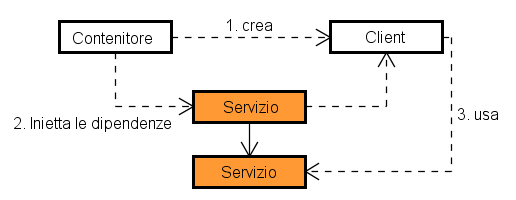
\includegraphics[scale=0.45]{UML/Package/strutturaPattern/DependencyInjection.png}
	\caption{Struttura logica del pattern Dependency Injection}
\end{figure}
\\
\textbf{Collaborazioni}
\\
\textbf{Svantaggi}	Eventuali errori legati alla risoluzione delle dipendenze o alla loro implementazione vengono rilevati solamente a \textit{runtime\ped{G}}.


\subsection{Comportamentali}
\subsubsection{Iterator}
\textbf{Scopo}
\textbf{Motivazione}
\textbf{Applicabilità}
\textbf{Utilizzo}
\textbf{Struttura}
\textbf{Collaborazioni}
\textbf{Svantaggi}
\subsubsection{Observer}
\textbf{Scopo}
\textbf{Motivazione}
\textbf{Applicabilità}
\textbf{Utilizzo}
\textbf{Struttura}
\textbf{Collaborazioni}
\textbf{Svantaggi}
\subsubsection{Strategy}
\textbf{Scopo}
\textbf{Motivazione}
\textbf{Applicabilità}
\textbf{Utilizzo}
\textbf{Struttura}
\textbf{Collaborazioni}
\textbf{Svantaggi}

\subsection{Architetturali}
\subsubsection{MVC}
\textbf{Scopo}
\textbf{Motivazione}
\textbf{Applicabilità}
\textbf{Utilizzo}
\textbf{Struttura}
\textbf{Collaborazioni}
\textbf{Svantaggi}
